\section{Evaluation}
\label{sec:evaluation}

\sys is implemented in three modules: a userspace library \libipc{} with $\approx$5000 lines of C/C++ code, a monitor program and  is divided to two parts: monitor and userspace library. Both parts are implemented in $\approx$5000 lines of C/C++ code. We take advantage of C++ templates for different types of queues in our design.

\subsection{Microbenchmarks}

Figure~\ref{fig:eval-conn-setup-tput} shows throughput of connection creation. Key points: a) FastSocket not fast enough, b) higher throughput, c) scalable with number of cores.

Figure~\ref{fig:eval-msgsize-intra} shows throughput and latency with different message sizes for intra-server communication. Key points: a) shared memory is faster than NIC hairpin, b) user space is faster than kernel, c) zero copy for large messages.

Figure~\ref{fig:eval-msgsize-inter} shows throughput and latency with different message sizes for inter-server communication. Key points: a) RDMA is faster than DPDK + user-space stack, b) zero copy for large messages.

Figure~\ref{fig:eval-connnum-tput} shows throughput with different number of concurrent connections (log scale on x axis). Key points: a) SocksDirect is scalable with number of connections, b) other systems with one queue per socket has performance degradation under high concurrency.

Figure~\ref{fig:eval-corenum-tput} shows throughput with different number of cores for intra-server communication. Key points: a) SocksDirect is scalable with number of cores, b) NIC hairpin is not scalable with number of cores.

Table~\ref{tab:eval-context-switch} shows throughput and latency with a dispatcher process on core $A$, multiple worker processes on core $B$ and a reducer process on core $C$. Key points: a) When all workers are active, throughput is comparable with single worker. b) When only a fraction of workers are active, the idle workers do not impact performance. c) Latency increases with number of active workers, but still much lower than Linux.

% Figure \ref{fig:eval-fork-tput} shows throughput and latency with \texttt{fork}. At time $T_0$, receiver forks, and the parent process keeps receiving. At time $T_1$, the child process begins to receives takes over the socket. At time $T_2$, sender forks, and only the parent sends. At time $T_3$, the child sender also starts sending.

\begin{figure}[htpb]
	\centering
	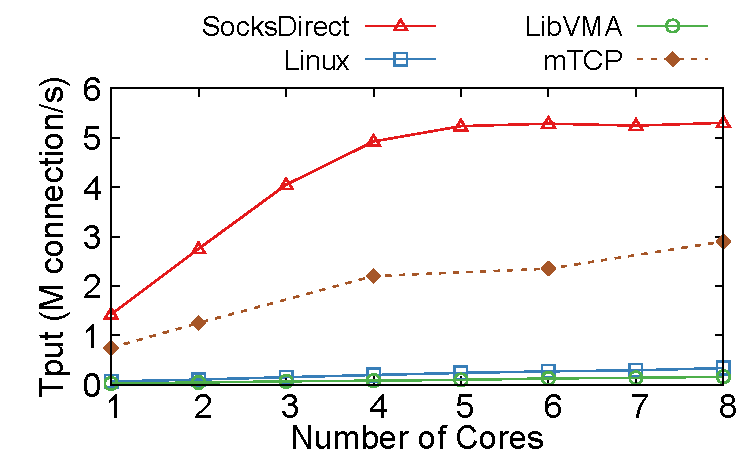
\includegraphics[width=0.33\textwidth]{eval/microbenchmark/conn-setup-tput.pdf}
	\caption{Throughput of the connection creation}
	\label{fig:eval-conn-setup-tput}
\end{figure}


\begin{figure}[htpb]
	\centering
	\subfloat[Intra-server throughput]{                    
		%\begin{minipage}{0.4\textwidth}
		\centering
		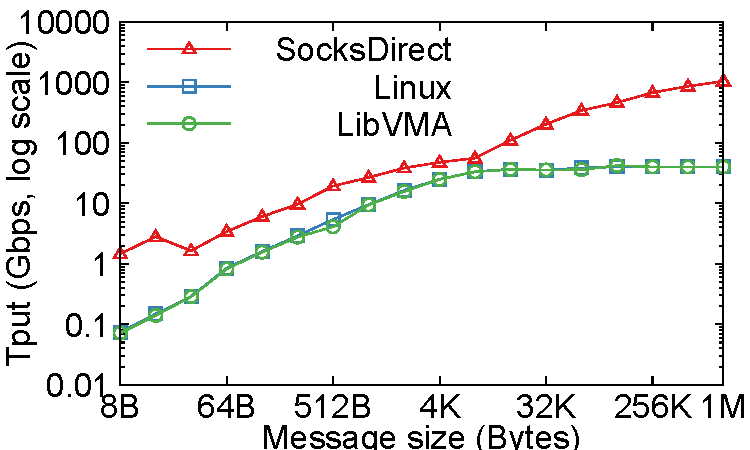
\includegraphics[width=0.33\textwidth]{eval/microbenchmark/msgsize-ipc-tput.pdf}
		\label{fig:eval-msgsize-ipc-tput}
		%\end{minipage}
	}
	
	\subfloat[Intra-server latency]{
		%\begin{minipage}{0.4\textwidth}
		\centering 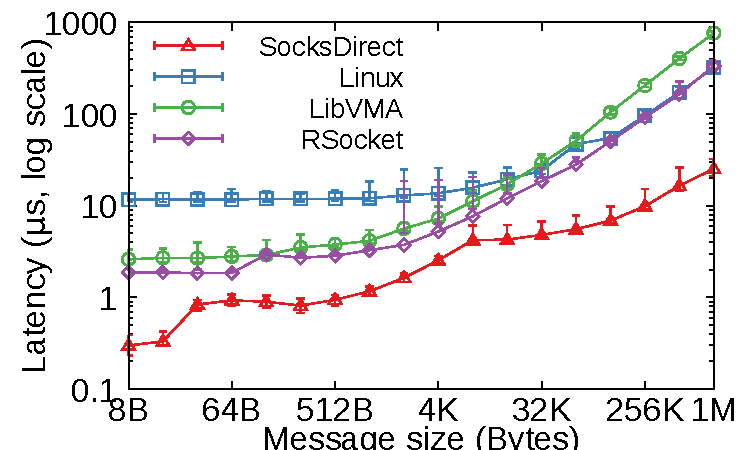
\includegraphics[width=0.33\textwidth]{eval/microbenchmark/msgsize-ipc-lat.pdf}
		\label{fig:eval-msgsize-ipc-lat}
		%\end{minipage}
	}
	\caption{Single-core intra-server performance with different message sizes.}
	\label{fig:eval-msgsize-intra}
\end{figure}

\begin{figure}[htpb]
	\centering
	\subfloat[Inter-server throughput]{
		%\begin{minipage}{0.4\textwidth}
		\centering 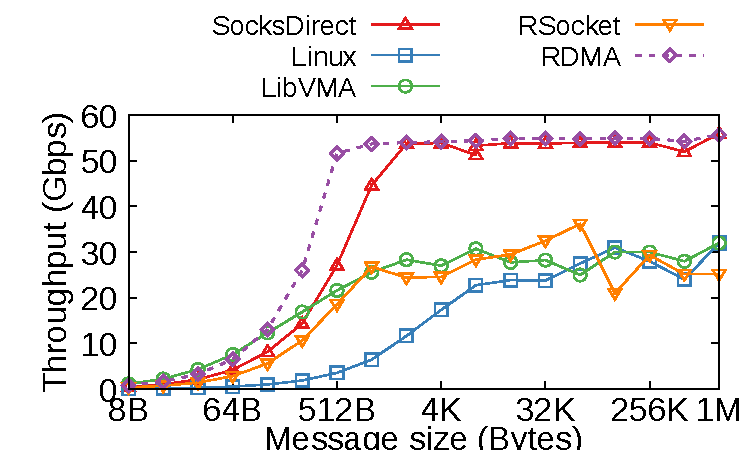
\includegraphics[width=0.33\textwidth]{eval/microbenchmark/msgsize-network-tput.pdf}
		\label{fig:eval-msgsize-network-tput}
		%\end{minipage}
	}
	
	\subfloat[Inter-server latency]{
		%\begin{minipage}{0.4\textwidth}
		\centering 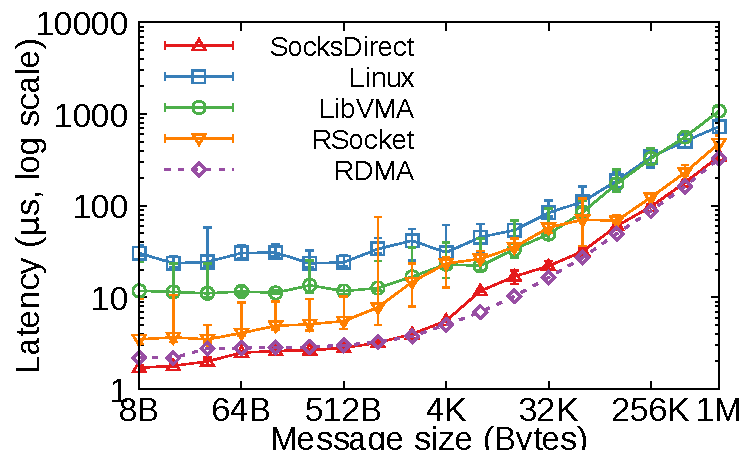
\includegraphics[width=0.33\textwidth]{eval/microbenchmark/msgsize-network-lat.pdf}
		\label{fig:eval-msgsize-network-lat}
		%\end{minipage}
	}
	\caption{Single-core inter-server performance with different message sizes.}
	\label{fig:eval-msgsize-inter}
\end{figure}

\begin{figure}[htpb]
\centering                                                         
\subfloat[Intra-server]{                    
	%\begin{minipage}{0.4\textwidth}
	    \centering
	    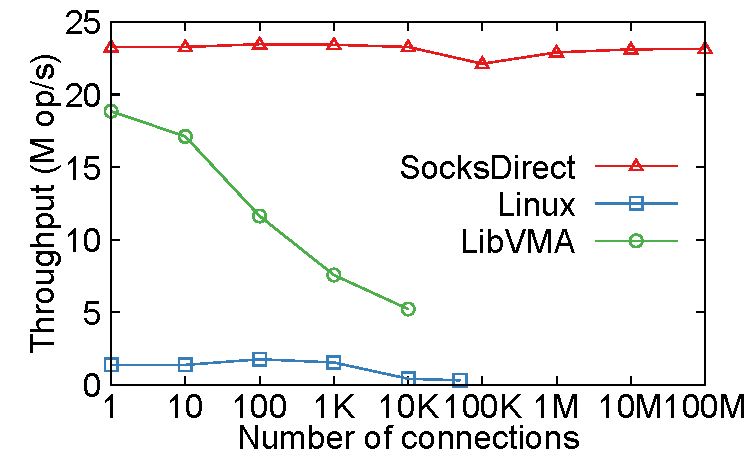
\includegraphics[width=0.33\textwidth]{eval/microbenchmark/connnum-ipc-tput.pdf}
	    \label{fig:eval-connnum-ipc-tput}
	%\end{minipage}
	}

\subfloat[Inter-server]{
	%\begin{minipage}{0.4\textwidth}
		\centering 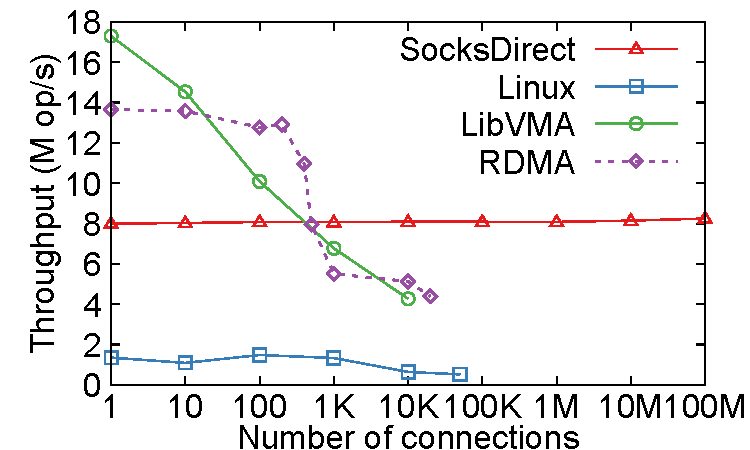
\includegraphics[width=0.33\textwidth]{eval/microbenchmark/connnum-network-tput.pdf}
		\label{fig:eval-connnum-network-tput}
	%\end{minipage}
	}
	\caption{Single-core throughput with different number of connections.}
	\label{fig:eval-connnum-tput}
\end{figure}

\begin{figure}[htpb]
	\subfloat[Intra-server]{                    
	%\begin{minipage}{0.4\textwidth}
	    \centering
	    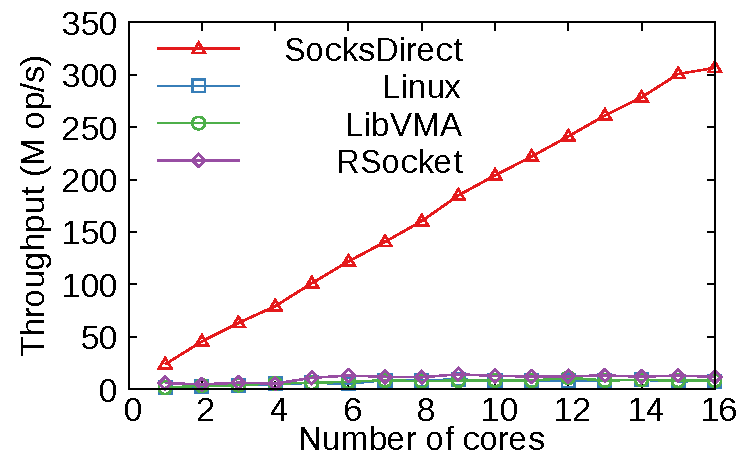
\includegraphics[width=0.33\textwidth]{eval/microbenchmark/corenum-IPC-tput.pdf}
	    \label{fig:eval-cornum-ipc}
	%\end{minipage}
	}

\subfloat[Inter-server]{
	%\begin{minipage}{0.4\textwidth}
		\centering 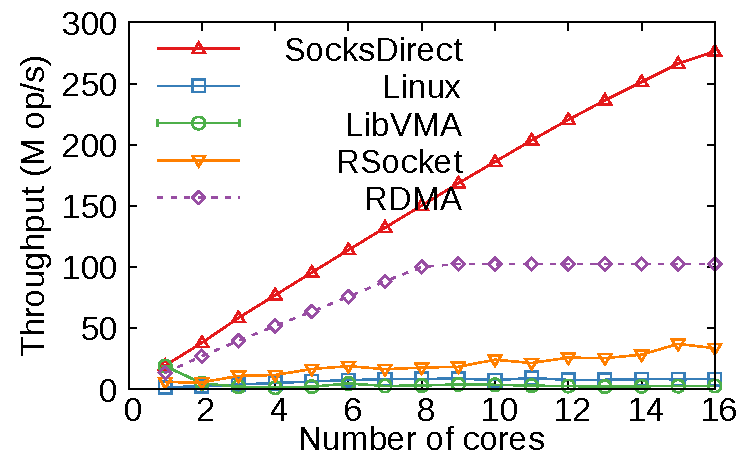
\includegraphics[width=0.33\textwidth]{eval/microbenchmark/corenum-network-tput.pdf}
		\label{fig:eval-cornum-network}
	%\end{minipage}
	}
	\caption{Throughput with different number of cores.}
	\label{fig:eval-corenum-tput}
\end{figure}


\begin{table}[t]
	\centering
		\begin{tabular}{l|c|c|c|c|c|c|}
			\hline
				& \multicolumn{3}{c|}{Throughput} & \multicolumn{3}{c|}{Latency} \\
			\hline
			Num of Workers	& \multicolumn{1}{c|}{1} & \multicolumn{2}{c|}{8} & \multicolumn{1}{c|}{1} & \multicolumn{2}{c|}{8} \\
			\hline
			Num of Active Workers	& 1 & 1 & 8 & 1 & 1 & 8 \\
			\hline
			\hline
			SocksDirect 	& 1 & 1 & 8 & 1 & 1 & 8 \\
			\hline
			Linux 	& 1 & 1 & 8 & 1 & 1 & 8 \\
			\hline
		\end{tabular}
	\caption{Performance evaluation of multiple processes sharing a core.}
	\label{tab:eval-context-switch}
\end{table}

%\begin{figure}[htpb]
%	\centering
%	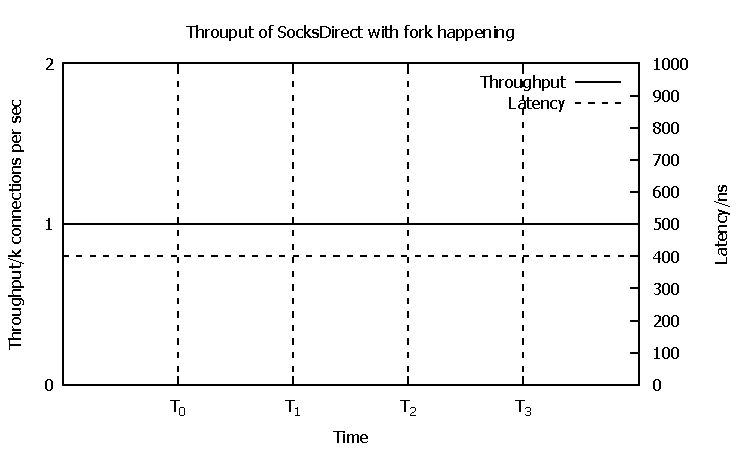
\includegraphics[width=\columnwidth]{eval/microbenchmark/fork-tput.pdf}
%	\caption{Throughput of SocksDirect with fork happening}
%	\label{fig:eval-fork-tput}
%\end{figure}


